\documentclass[a4paper, 12pt]{article}
\usepackage{comment} % enables the use of multi-line comments (\ifx \fi)
\usepackage{graphicx}
\usepackage{fullpage} % changes the margin
\usepackage{listings}
\usepackage{xparse}
\usepackage{xcolor}
\usepackage{minted}
\usepackage{amsmath}
\usepackage{varwidth}
\usepackage{tikz}

\usetikzlibrary{shapes,arrows,automata}

\tikzstyle{block} = [draw, fill=blue!20, rectangle, 
    minimum height=3em, minimum width=6em]
\tikzstyle{sum} = [draw, fill=blue!20, circle, node distance=1cm]
\tikzstyle{input} = [coordinate]
\tikzstyle{output} = [coordinate]
\tikzstyle{pinstyle} = [pin edge={to-,thin,black}]

\NewDocumentCommand{\codeword}{v}{%
\texttt{\textcolor{blue}{#1}}%
}

\newcommand{\block}[1]{%
  \begingroup
  \setlength{\fboxsep}{0pt}%
  \vrule width0pt height \blockdim
  \ooalign{%
    \framebox[\blockdim]{\rule{0pt}{\blockdim}}\cr
    \hidewidth\raisebox{0.5\dimexpr\blockdim-\height}{\raisebox{\depth}{#1}}\hidewidth\cr
  }%
  \endgroup
}
\newcommand{\joinblocks}{\unskip\kern-\fboxrule\ignorespaces}
\newenvironment{blocks}[1][1cm]
 {\begin{varwidth}{\textwidth}\setlength{\blockdim}{#1}\makeblocks}
 {\end{varwidth}}
\newcommand{\makeblocks}{%
  \begingroup\lccode`~=`&\lowercase{\endgroup\let~}\joinblocks
  \catcode`\&=\active
  \baselineskip=0pt
  \lineskiplimit=\maxdimen
  \lineskip=0pt
  \centering
}
\newlength{\blockdim}

\begin{document}
% Header
\noindent
\LARGE\textbf{Intrastellar} \hfill \\
\newline
\large\textbf{Preliminary Design Report} \hfill \textbf{Zach Schuermann} \\
\normalsize ECE 4273-001 \hfill 112944063 \\
Dr. Erik Petrich \hfill Date: 04/16/19 

\section*{Project Objectives}
The ultimate goal for this project is to create a retro video game using the LPC1769 and supporting hardware. I have elected to create a Galaga-like game implemented on an LPC1769 with a Playstation 2 controller for user input/control and a 480x800 LCD display. The gameplay will be in real-time with the goal of destroying enemies (like Galaga) or asteroids. In general, there are three main subsystems: display, controller input, and sound. The game will continuously poll controller input, implement game logic, render the screen (via the display driver), and synthesize sound when necessary. The implementation is discussed below. 

\section*{Project Design}
Initial construction of the project is shown in Figure \ref{fig:pic}. The project will implement the following features:

\begin{center}
  \begin{tabular}{ |c|c|c| }
    \hline
    \textbf{Component} & \textbf{Description} & \textbf{Points} \\
    \hline
    \hline
    Game Type & Animated real-time game (objects continuously in motion) & 2 \\
    \hline
    Display & Use a graphical LCD for output  & 2 \\
    \hline
    Input & Use a game controller with a serial interface (Playstation 2) & 0.5 \\ 
    \hline
    Sound & Use D-to-A to generate a sine wave based sound effect  & 1 \\
    \hline
    Other & Use non-volatile memory (EEPROM  to retain high score table) & 0.5 \\ 
    \hline
    Total & & 6 \\ 
    \hline
  \end{tabular}
\end{center}

\begin{figure}[h!]
  \centering
  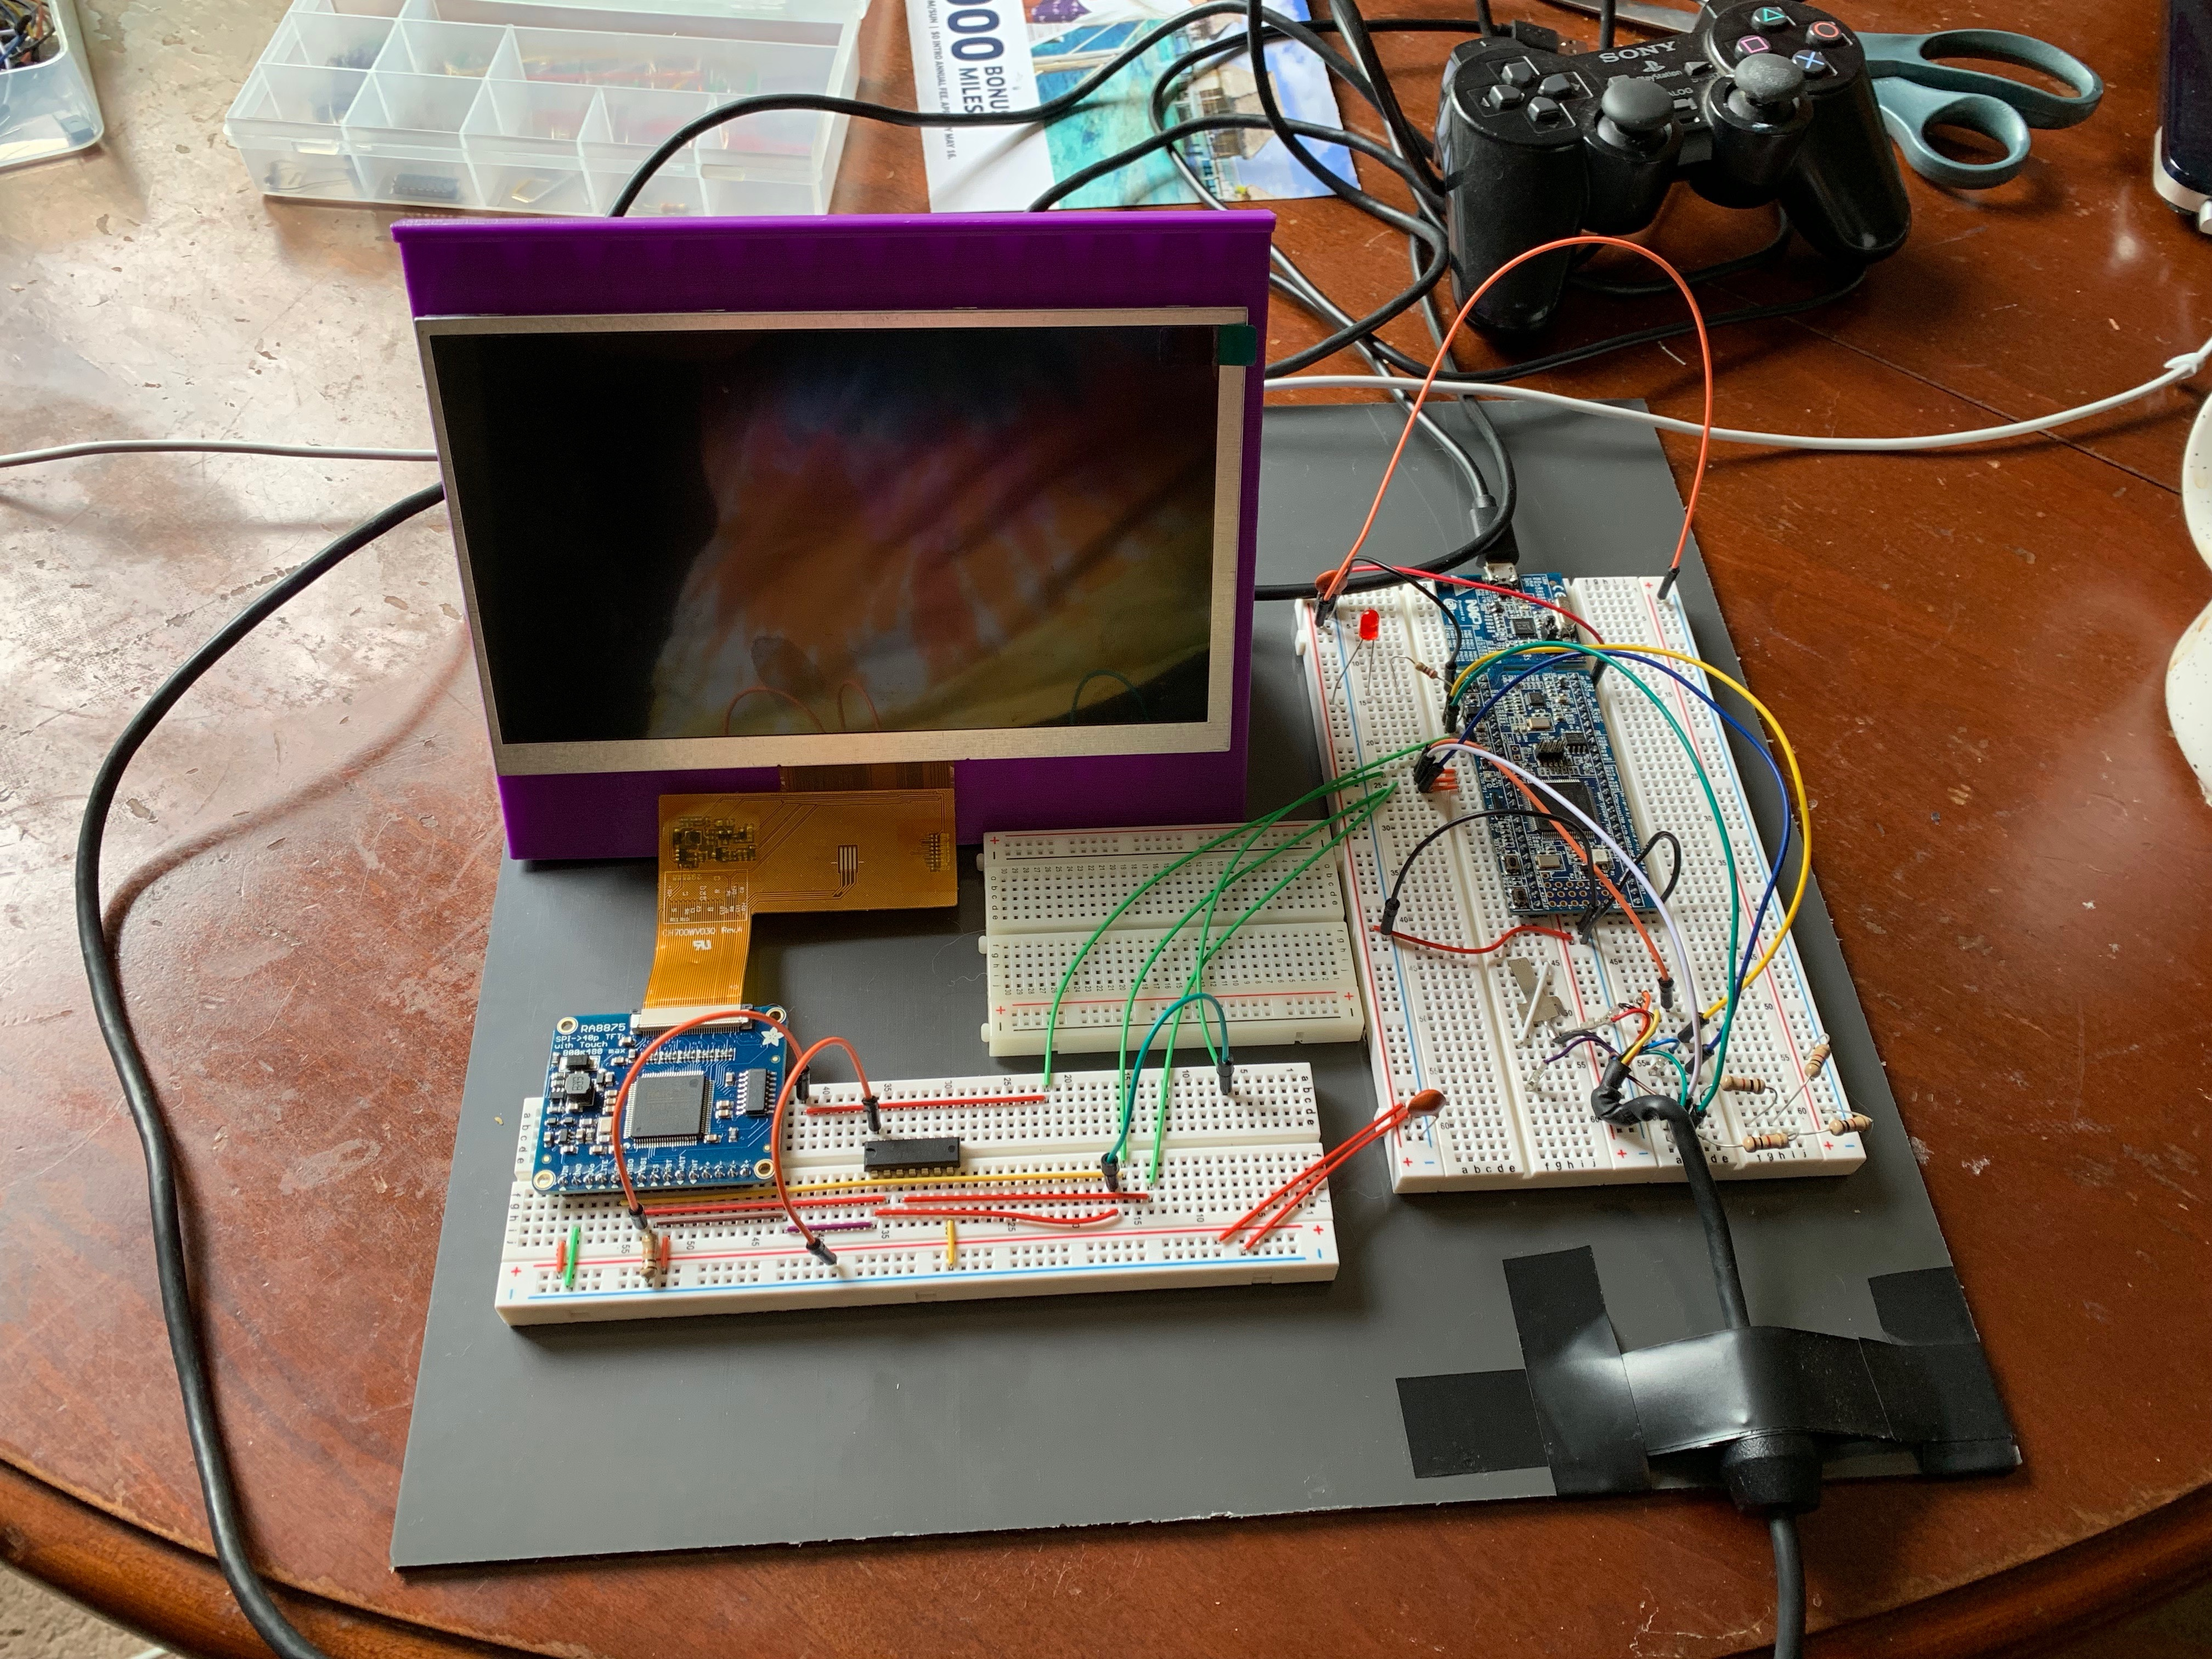
\includegraphics[scale=.1]{pic.png}
  \caption{Preliminary Implementation}
  \label{fig:pic}
\end{figure}

\subsection*{Display Sub-System}
The display subsystem relies on an Adafruit 40-pin LCD 480x800 7" display. In order to effectively communicate with such a large display, an intermediate processor is utilized. The Adafruit RA8875 Display Driver Board was selected as a sufficient intermediary. The board has 768 kB of memory to store the entire frame buffer, and is easily changed via SPI. Furthermore, there are a number of hardware-accelerated functions for drawing specific shapes. This system will likely utilize a 2-4 MHz SPI clock. 

\subsection*{Controller Sub-System}
The Playstation 2 (PS2) controller will act as the means for the user to control the game. The PS2 controller uses a serial protocol which is essentially SPI. In order to communicate, the clock rate will require decreasing to about 250 kHz. 

\subsection*{Sound Sub-System}
The sound will be generated via the D-to-A system onboard the LPC1769. Sine wave-based signals will be synthesized for music, sound effects, or both. The waveform generated will be output to an LM386 audio operational amplifier in order to drive a loudspeaker. A potentiometer will act as volume control through voltage division of the pre-amplified signal. 

\subsection*{EEPROM}
Lastly, the design relies on the onboard EEPROM to save the high score to a location which will not change on power cycling. This system is already implemented on the LPCXpresso development board via the I2C subsystem.  

\section*{Hardware Design}

\begin{figure}[h!]
  \centering
  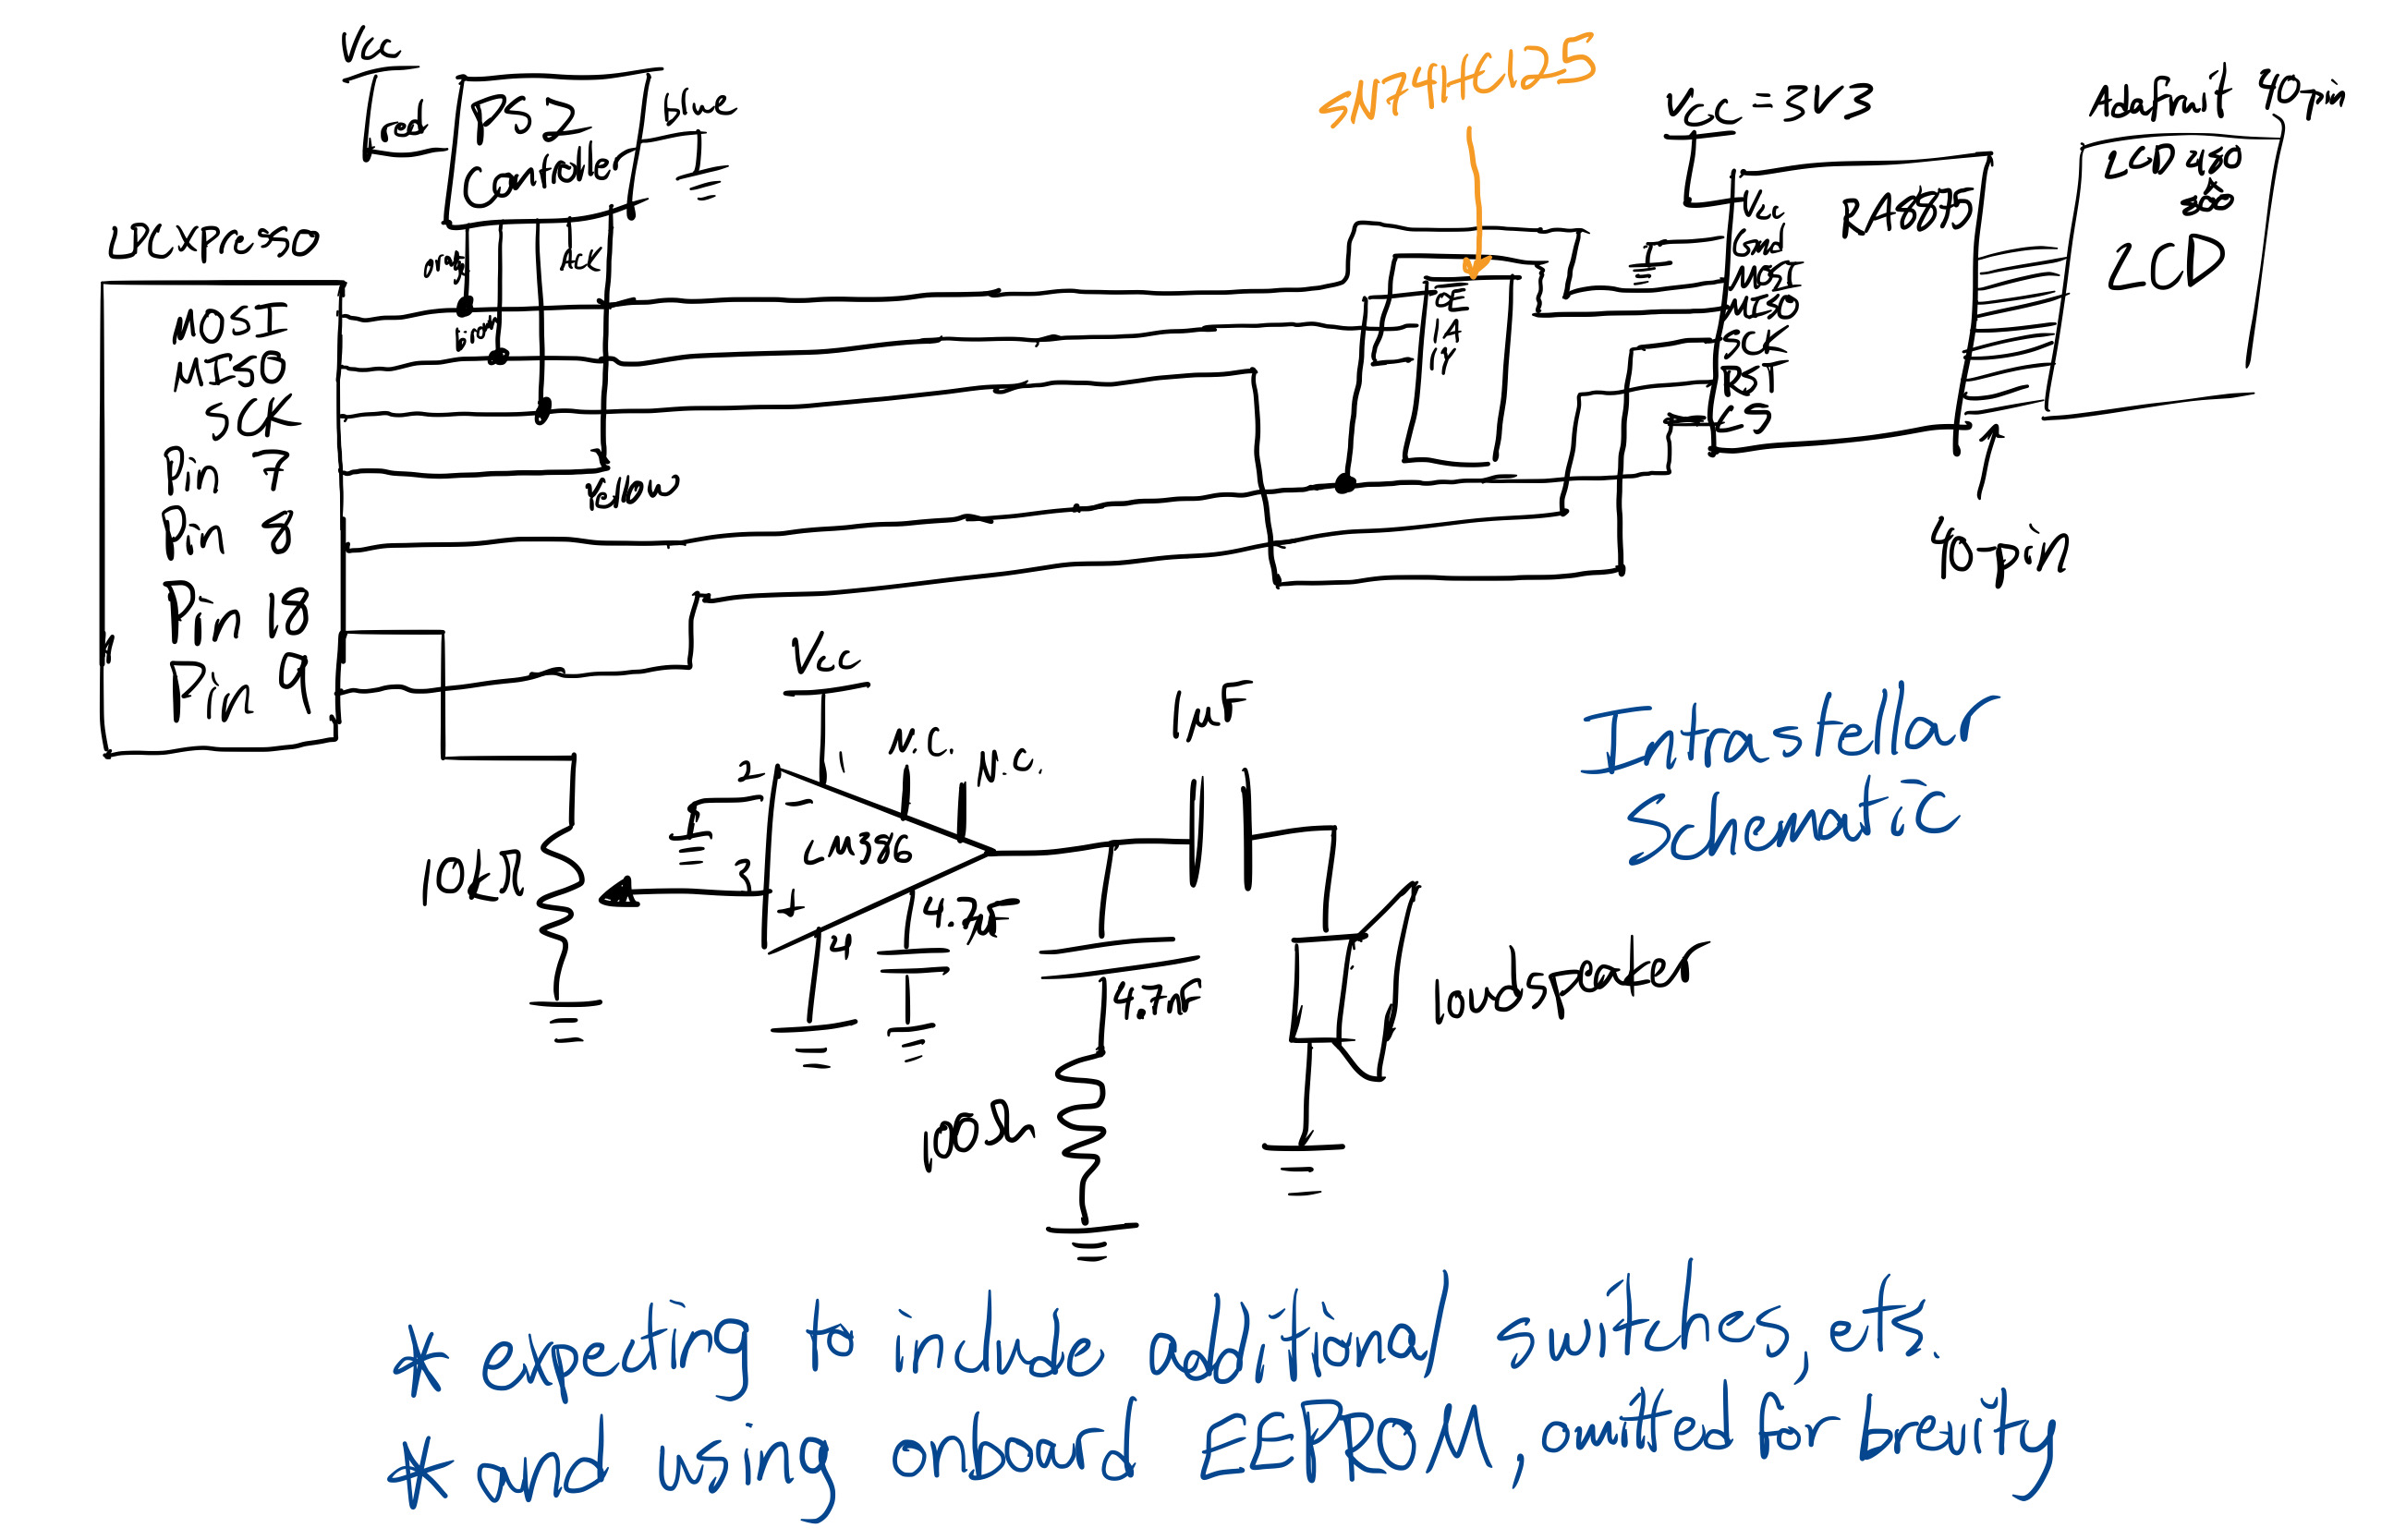
\includegraphics[scale=.18]{schematic.png}
  \caption{Preliminary Hardware Schematic}
  \label{fig:schematic}
\end{figure}

The schematic in Figure \ref{fig:schematic} illustrates the hardware design for the project. 

\section*{Software Design}
The software is partially implemented, and the source is included at the end of the report. The general design includes the implementation of the Adafruit RA8875 library for our microcontroller, game logic, sound generation, and controller communication. The many subsystems referenced above will require configuring through software. Furthermore, the processor will be clocked at 96 MHz in order to provide for sufficient speed for SPI communication as well as executing game logic and rendering quickly. Aside from configuration and communication, the software will enter a game loop which will continuously poll the controller for input, implement the game logic, and render the output. This will likely be decomposed into a number of subtasks -- some of which will require implementation with interrupts. The source right now is contained in a single file, but will be migrated to multiple source files/headers for final implementation. 

\begin{minted}{c}
/*
===============================================================================
 Name        : intrastellar.c
 Author      : Zach Schuermann
 Version     :
 Copyright   : Zach Schuermann, 2019
 Description : Intrastellar Retro Game
===============================================================================
*/

#ifdef __USE_CMSIS
#include "LPC17xx.h"
#endif

#include <cr_section_macros.h>
#include <stdint.h>

//#define uint8_t unsigned char

uint8_t lcd_read_data();
void spi_begin();
/* Text functions */
void    lcd_text_mode(void);
void    lcd_text_set_cursor(uint16_t x, uint16_t y);
void    lcd_text_color(uint16_t foreColor, uint16_t bgColor);
void    lcd_text_transparent(uint16_t foreColor);
//void    textEnlarge(uint8_t scale);
void    lcd_text_write(const char* buffer, uint16_t len);
void    lcd_cursor_blink(uint8_t rate);

/* Low level access */
void    lcd_write_reg(uint8_t reg, uint8_t val);
uint8_t lcd_read_reg(uint8_t reg);
void    lcd_write_data(uint8_t d);
uint8_t lcd_read_data(void);
void    lcd_write_command(uint8_t d);
uint8_t lcd_read_status(void);



// Colors (RGB565)
#define	RA8875_BLACK            0x0000 ///< Black Color
#define	RA8875_BLUE             0x001F ///< Blue Color
#define	RA8875_RED              0xF800 ///< Red Color
#define	RA8875_GREEN            0x07E0 ///< Green Color
#define RA8875_CYAN             0x07FF ///< Cyan Color
#define RA8875_MAGENTA          0xF81F ///< Magenta Color
#define RA8875_YELLOW           0xFFE0 ///< Yellow Color
#define RA8875_WHITE            0xFFFF ///< White Color

// Command/Data pins for SPI
#define RA8875_DATAWRITE        0x00
#define RA8875_DATAREAD         0x40
#define RA8875_CMDWRITE         0x80
#define RA8875_CMDREAD          0xC0

// Registers & bits
#define RA8875_PWRR             0x01
#define RA8875_PWRR_DISPON      0x80
#define RA8875_PWRR_DISPOFF     0x00
#define RA8875_PWRR_SLEEP       0x02
#define RA8875_PWRR_NORMAL      0x00
#define RA8875_PWRR_SOFTRESET   0x01

#define RA8875_MRWC             0x02

#define RA8875_GPIOX            0xC7

#define RA8875_PLLC1            0x88
#define RA8875_PLLC1_PLLDIV2    0x80
#define RA8875_PLLC1_PLLDIV1    0x00

#define RA8875_PLLC2            0x89
#define RA8875_PLLC2_DIV1       0x00
#define RA8875_PLLC2_DIV2       0x01
#define RA8875_PLLC2_DIV4       0x02
#define RA8875_PLLC2_DIV8       0x03
#define RA8875_PLLC2_DIV16      0x04
#define RA8875_PLLC2_DIV32      0x05
#define RA8875_PLLC2_DIV64      0x06
#define RA8875_PLLC2_DIV128     0x07

#define RA8875_SYSR             0x10
#define RA8875_SYSR_8BPP        0x00
#define RA8875_SYSR_16BPP       0x0C
#define RA8875_SYSR_MCU8        0x00
#define RA8875_SYSR_MCU16       0x03

#define RA8875_PCSR             0x04
#define RA8875_PCSR_PDATR       0x00
#define RA8875_PCSR_PDATL       0x80
#define RA8875_PCSR_CLK         0x00
#define RA8875_PCSR_2CLK        0x01
#define RA8875_PCSR_4CLK        0x02
#define RA8875_PCSR_8CLK        0x03

#define RA8875_HDWR             0x14

#define RA8875_HNDFTR           0x15
#define RA8875_HNDFTR_DE_HIGH   0x00
#define RA8875_HNDFTR_DE_LOW    0x80

#define RA8875_HNDR             0x16
#define RA8875_HSTR             0x17
#define RA8875_HPWR             0x18
#define RA8875_HPWR_LOW         0x00
#define RA8875_HPWR_HIGH        0x80

#define RA8875_VDHR0            0x19
#define RA8875_VDHR1            0x1A
#define RA8875_VNDR0            0x1B
#define RA8875_VNDR1            0x1C
#define RA8875_VSTR0            0x1D
#define RA8875_VSTR1            0x1E
#define RA8875_VPWR             0x1F
#define RA8875_VPWR_LOW         0x00
#define RA8875_VPWR_HIGH        0x80

#define RA8875_HSAW0            0x30
#define RA8875_HSAW1            0x31
#define RA8875_VSAW0            0x32
#define RA8875_VSAW1            0x33

#define RA8875_HEAW0            0x34
#define RA8875_HEAW1            0x35
#define RA8875_VEAW0            0x36
#define RA8875_VEAW1            0x37

#define RA8875_MCLR             0x8E
#define RA8875_MCLR_START       0x80
#define RA8875_MCLR_STOP        0x00
#define RA8875_MCLR_READSTATUS  0x80
#define RA8875_MCLR_FULL        0x00
#define RA8875_MCLR_ACTIVE      0x40

#define RA8875_DCR                    0x90
#define RA8875_DCR_LINESQUTRI_START   0x80
#define RA8875_DCR_LINESQUTRI_STOP    0x00
#define RA8875_DCR_LINESQUTRI_STATUS  0x80
#define RA8875_DCR_CIRCLE_START       0x40
#define RA8875_DCR_CIRCLE_STATUS      0x40
#define RA8875_DCR_CIRCLE_STOP        0x00
#define RA8875_DCR_FILL               0x20
#define RA8875_DCR_NOFILL             0x00
#define RA8875_DCR_DRAWLINE           0x00
#define RA8875_DCR_DRAWTRIANGLE       0x01
#define RA8875_DCR_DRAWSQUARE         0x10

#define RA8875_ELLIPSE                0xA0
#define RA8875_ELLIPSE_STATUS         0x80

#define RA8875_MWCR0            0x40
#define RA8875_MWCR0_GFXMODE    0x00
#define RA8875_MWCR0_TXTMODE    0x80
#define RA8875_MWCR0_CURSOR     0x40
#define RA8875_MWCR0_BLINK      0x20

#define RA8875_MWCR0_DIRMASK    0x0C ///< Bitmask for Write Direction
#define RA8875_MWCR0_LRTD       0x00 ///< Left->Right then Top->Down
#define RA8875_MWCR0_RLTD       0x04 ///< Right->Left then Top->Down
#define RA8875_MWCR0_TDLR       0x08 ///< Top->Down then Left->Right
#define RA8875_MWCR0_DTLR       0x0C ///< Down->Top then Left->Right

#define RA8875_BTCR             0x44
#define RA8875_CURH0            0x46
#define RA8875_CURH1            0x47
#define RA8875_CURV0            0x48
#define RA8875_CURV1            0x49

#define RA8875_P1CR             0x8A
#define RA8875_P1CR_ENABLE      0x80
#define RA8875_P1CR_DISABLE     0x00
#define RA8875_P1CR_CLKOUT      0x10
#define RA8875_P1CR_PWMOUT      0x00

#define RA8875_P1DCR            0x8B

#define RA8875_P2CR             0x8C
#define RA8875_P2CR_ENABLE      0x80
#define RA8875_P2CR_DISABLE     0x00
#define RA8875_P2CR_CLKOUT      0x10
#define RA8875_P2CR_PWMOUT      0x00

#define RA8875_P2DCR            0x8D

#define RA8875_PWM_CLK_DIV1     0x00
#define RA8875_PWM_CLK_DIV2     0x01
#define RA8875_PWM_CLK_DIV4     0x02
#define RA8875_PWM_CLK_DIV8     0x03
#define RA8875_PWM_CLK_DIV16    0x04
#define RA8875_PWM_CLK_DIV32    0x05
#define RA8875_PWM_CLK_DIV64    0x06
#define RA8875_PWM_CLK_DIV128   0x07
#define RA8875_PWM_CLK_DIV256   0x08
#define RA8875_PWM_CLK_DIV512   0x09
#define RA8875_PWM_CLK_DIV1024  0x0A
#define RA8875_PWM_CLK_DIV2048  0x0B
#define RA8875_PWM_CLK_DIV4096  0x0C
#define RA8875_PWM_CLK_DIV8192  0x0D
#define RA8875_PWM_CLK_DIV16384 0x0E
#define RA8875_PWM_CLK_DIV32768 0x0F

#define RA8875_TPCR0                  0x70
#define RA8875_TPCR0_ENABLE           0x80
#define RA8875_TPCR0_DISABLE          0x00
#define RA8875_TPCR0_WAIT_512CLK      0x00
#define RA8875_TPCR0_WAIT_1024CLK     0x10
#define RA8875_TPCR0_WAIT_2048CLK     0x20
#define RA8875_TPCR0_WAIT_4096CLK     0x30
#define RA8875_TPCR0_WAIT_8192CLK     0x40
#define RA8875_TPCR0_WAIT_16384CLK    0x50
#define RA8875_TPCR0_WAIT_32768CLK    0x60
#define RA8875_TPCR0_WAIT_65536CLK    0x70
#define RA8875_TPCR0_WAKEENABLE       0x08
#define RA8875_TPCR0_WAKEDISABLE      0x00
#define RA8875_TPCR0_ADCCLK_DIV1      0x00
#define RA8875_TPCR0_ADCCLK_DIV2      0x01
#define RA8875_TPCR0_ADCCLK_DIV4      0x02
#define RA8875_TPCR0_ADCCLK_DIV8      0x03
#define RA8875_TPCR0_ADCCLK_DIV16     0x04
#define RA8875_TPCR0_ADCCLK_DIV32     0x05
#define RA8875_TPCR0_ADCCLK_DIV64     0x06
#define RA8875_TPCR0_ADCCLK_DIV128    0x07

#define RA8875_TPCR1            0x71
#define RA8875_TPCR1_AUTO       0x00
#define RA8875_TPCR1_MANUAL     0x40
#define RA8875_TPCR1_VREFINT    0x00
#define RA8875_TPCR1_VREFEXT    0x20
#define RA8875_TPCR1_DEBOUNCE   0x04
#define RA8875_TPCR1_NODEBOUNCE 0x00
#define RA8875_TPCR1_IDLE       0x00
#define RA8875_TPCR1_WAIT       0x01
#define RA8875_TPCR1_LATCHX     0x02
#define RA8875_TPCR1_LATCHY     0x03

#define RA8875_TPXH             0x72
#define RA8875_TPYH             0x73
#define RA8875_TPXYL            0x74

#define RA8875_INTC1            0xF0
#define RA8875_INTC1_KEY        0x10
#define RA8875_INTC1_DMA        0x08
#define RA8875_INTC1_TP         0x04
#define RA8875_INTC1_BTE        0x02

#define RA8875_INTC2            0xF1
#define RA8875_INTC2_KEY        0x10
#define RA8875_INTC2_DMA        0x08
#define RA8875_INTC2_TP         0x04
#define RA8875_INTC2_BTE        0x02

#define RA8875_SCROLL_BOTH      0x00
#define RA8875_SCROLL_LAYER1    0x40
#define RA8875_SCROLL_LAYER2    0x80
#define RA8875_SCROLL_BUFFER    0xC0

// GPIO
#define FIO0DIR (*(volatile unsigned int *) 0x2009c000)
#define FIO0PIN (*(volatile unsigned int *) 0x2009c014)
#define FIO3DIR (*(volatile unsigned int *) 0x2009c060)
#define FIO3PIN (*(volatile unsigned int *) 0x2009c074)
#define PINSEL0 (*(volatile unsigned int *) 0x4002C000)
#define PINSEL1 (*(volatile unsigned int *) 0x4002C004)

// clock
#define CLKOUTCFG   (*(volatile unsigned int *) 0x400fc1c8)
#define PLL0CON     (*(volatile unsigned int *) 0x400FC080)
#define PLL0CFG     (*(volatile unsigned int *) 0x400FC084)
#define PLL0FEED    (*(volatile unsigned int *) 0x400FC08C)
#define PLL0STAT    (*(volatile unsigned int *) 0x400FC088)
#define CCLKCFG     (*(volatile unsigned int *) 0x400FC104)
#define PCLKSEL0 	(*(volatile unsigned int *) 0x400FC1A8)

// SPI
#define S0SPCCR		(*(volatile unsigned int *) 0x4002000C)
#define S0SPCR 		(*(volatile unsigned int *) 0x40020000)
#define S0SPSR 		(*(volatile unsigned int *) 0x40020004)
#define S0SPDR		(*(volatile unsigned int *) 0x40020008)

// I2C
#define I2C1CONSET 	(*(volatile unsigned int *) 0x4005C000)
#define I2C1CONCLR 	(*(volatile unsigned int *) 0x4005C018)
#define I2C1DAT 	(*(volatile unsigned int *) 0x4005C008)
#define I2C1STAT 	(*(volatile unsigned int *) 0x4005C004)
#define I2C1SCLH 	(*(volatile unsigned int *) 0x4005C010)
#define I2C1SCLL 	(*(volatile unsigned int *) 0x4005C014)

// Systick
#define STCTRL		(*(volatile unsigned int *) 0xE000E010)
#define STRELOAD	(*(volatile unsigned int *) 0xE000E014)

void wait_ticks(int count) {
    volatile int ticks = count;
    while (ticks > 0)
        ticks--;
}

/*
 * setup CPU clock for 96 MHz instead of default 4MHz
 * using PLL0 and IRC oscillator
 */
void clock_setup(void) {
	// select P1.27 for clock out and enable
	// PINSEL3 |= (1<<22);
	CLKOUTCFG = (1<<8);

	// bit 0 enable, bit 1 connect
	PLL0CON = 0;
	// PLL0 setup
	// feed sequence - disconnect
	PLL0FEED = 0xAA;
	PLL0FEED = 0x55;

	// Generate 288MHz with 36x multiplier
	PLL0CFG = 0x23;
	PLL0FEED = 0xAA;
	PLL0FEED = 0x55;

	//enable
	PLL0CON = 0x1;
	PLL0FEED = 0xAA;
	PLL0FEED = 0x55;

	// Divide by 3 to get 96MHz
	CCLKCFG = 0x2;

	// wait for lock
    while(!((PLL0STAT & (1<<26)) >> 26)) {}

    // connect
    PLL0CON = 0x3;
    PLL0FEED = 0xAA;
    PLL0FEED = 0x55;
}

void gpio_setup() {
	// LED Setup
	FIO0DIR |= (1<<22);
	FIO3DIR |= (3<<25);

	// SPI SS
	FIO0DIR |= (1<<9); // P0.9 is SS for PS2
	FIO0DIR |= (1<<7); // P0.7 is SS for LCD
	FIO0DIR |= (1<<6); // P0.6 is RST for LCD
}

void spi_setup() {
	PINSEL0 |= (3 << 30); // SCK
	PINSEL1 |= (3 << 2); // MISO
	PINSEL1 |= (3 << 4); // MOSI
}

void ps2_spi_setup() {
	// 96 MHz / 8 => 12 MHz SPI clock
	PCLKSEL0 |= (3<<16);

	// 12 MHz / 48 => 250kHz SCK
	S0SPCCR |= 0x30;

	// phase
	S0SPCR |= (1<<3);

	// active low clock
	S0SPCR |= (1<<4);

	// operate in master mode
	S0SPCR |= (1<<5);

	// LSB first
	S0SPCR |= (1<<6);
}

void lcd_spi_setup() {
	// 96 MHz / 8 => 12 MHz SPI clock (11)
	// 96 / 2 => 48 MHz (10)
	PCLKSEL0 &= ~(1<<16);
	PCLKSEL0 &= ~(1<<17); // was high

	// 48 MHz / 12 => 4 MHz SCK
	// has to be even, >= 8
	S0SPCCR = 0xC;

	// phase (default)
	S0SPCR |= (1<<3);

	// active low clock
	S0SPCR |= (1<<4);

	// operate in master mode
	S0SPCR |= (1<<5);

	// MSB first (default)
	S0SPCR &= ~(1<<6);
	wait_ticks(100);
}

void interrupt_setup() {
	STRELOAD = 100000;
	STCTRL = 0b111;
}

void led(int num) {
	if(num == -1) {
		FIO3PIN |= (1<<25);
		FIO3PIN |= (1<<26);
		FIO0PIN |= (1<<22);
	}
	else if(num == 0) {
		FIO3PIN |= (1<<25);
		FIO3PIN |= (1<<26);
		FIO0PIN &= ~(1<<22); // turn on red
	}
	else if (num == 1) {
		FIO0PIN |= (1<<22); // turn off LED
		FIO3PIN |= (1<<26);
		FIO3PIN &= ~(1<<25); // turn on green
	}
	else {
		FIO0PIN |= (1<<22); // turn off LED
		FIO3PIN |= (1<<25);
		FIO3PIN &= ~(1<<26); // turn on blue
	}
}

/*
 * clock test - run for 5 seconds - default 4MHz counts to ~2MM,
 * 96 MHz counts to ~49MM
 */
void clock_test() {
	// Force the counter to be placed into memory
	volatile static int i = 0;

	// Enter an infinite loop, just incrementing a counter
	while(1) {
		i++ ;
	}
}

int read_controller() {
	int controller = 0;
	volatile int status;
	int read;

	// new packet assert SS
	FIO0PIN &= ~(1<<9);

	//// START HEADER ////
	S0SPDR = 0x01;
	while((S0SPSR & (1<<7)) == 0) {}
	status = S0SPSR;
	//int read0 = S0SPDR; //FF
	read = S0SPDR;

	S0SPDR = 0x42;
	while((S0SPSR & (1<<7)) == 0) {}
	status = S0SPSR;
	//int read1 = S0SPDR; //FF
	read = S0SPDR;

	S0SPDR = 0x00;
	while((S0SPSR & (1<<7)) == 0) {}
	status = S0SPSR;
	//int read2 = S0SPDR; //41
	read = S0SPDR;

	S0SPDR = 0x00;
	while((S0SPSR & (1<<7)) == 0) {}
	status = S0SPSR;
	//int read3 = S0SPDR; //5A
	read = S0SPDR;
	//// END HEADER ////

	//// DIGITAL ////
	S0SPDR = 0x00;
	while((S0SPSR & (1<<7)) == 0) {}
	status = S0SPSR;
	//int read4 = S0SPDR; //0xFF -> 0xEF up pad
	read = S0SPDR;
	controller |= (read ^ 0xff) << 24;

	S0SPDR = 0x00;
	while((S0SPSR & (1<<7)) == 0) {}
	status = S0SPSR;
	//int read5 = S0SPDR; //0xFF unpressed -> 7F square
	read = S0SPDR;
	controller |= (read ^ 0xff) << 16;
	//// END DIGITAL ////

	//////UNUSED///////
	//// RIGHT JOY ////
	S0SPDR = 0x00;
	while((S0SPSR & (1<<7)) == 0) {}
	status = S0SPSR;
	//int read6 = S0SPDR; //0x83 unpressed
	read = S0SPDR;
	S0SPDR = 0x00;
	while((S0SPSR & (1<<7)) == 0) {}
	status = S0SPSR;
	//int read7 = S0SPDR; //0x83 unpressed
	read = S0SPDR;
	//// END RIGHT ////
	///////////////////

	//// LEFT JOY ////
	// X
	S0SPDR = 0x00;
	while((S0SPSR & (1<<7)) == 0) {}
	status = S0SPSR;
	//int read8 = S0SPDR; //0x7C unpressed, 0x00 left, 0xff right
	read = S0SPDR;
	controller |= read << 8;
	// Y
	S0SPDR = 0x00;
	while((S0SPSR & (1<<7)) == 0) {}
	status = S0SPSR;
	//int read9 = S0SPDR; //0x6E unpressed 0x00 top, 0xff bottom
	read = S0SPDR;
	controller |= read;
	//// END LEFT ////

	// de-assert SS
	FIO0PIN |= (1<<9);

	return controller;
}

void lcd_select() {
	FIO0PIN &= ~(1<<7);
}

void lcd_free() {
	FIO0PIN |= (1<<7);
}

void spi_begin() {
	lcd_spi_setup();
}

uint8_t spi_send(uint8_t data) {
	S0SPDR = data;
	while((S0SPSR & (1<<7)) == 0) {}
	volatile int status = S0SPSR;
	volatile int read = S0SPDR;
	//while(1) {}
	return read;
}

void spi_end() {

}

/**************************************************************************/
/*!
    Write data to the specified register

    @param reg Register to write to
    @param val Value to write
*/
/**************************************************************************/
void lcd_write_reg(uint8_t reg, uint8_t val) {
	lcd_write_command(reg);
	lcd_write_data(val);
}

/**************************************************************************/
/*
    Set the register to read from

    @param reg Register to read

    @return The value
*/
/**************************************************************************/
uint8_t lcd_read_reg(uint8_t reg) {
	lcd_write_command(reg);
	return lcd_read_data();
}

/**************************************************************************/
/*!
    Write data to the current register

    @param d Data to write
*/
/**************************************************************************/
void lcd_write_data(uint8_t d)
{
	lcd_select();
	spi_begin();
	spi_send(RA8875_DATAWRITE);
	spi_send(d);
	spi_end();
	lcd_free();
}

/**************************************************************************/
/*!
    Read the data from the current register

    @return The Value
*/
/**************************************************************************/
uint8_t lcd_read_data(void)
{
	lcd_select();
	spi_begin();
	spi_send(RA8875_DATAREAD);
	uint8_t x = spi_send(0x0);
	spi_end();
	lcd_free();
	return x;
}

/**************************************************************************/
/*!
    Write a command to the current register

    @param d The data to write as a command
 */
/**************************************************************************/
void lcd_write_command(uint8_t d)
{
	lcd_select();
	spi_begin();
	spi_send(RA8875_CMDWRITE);
	spi_send(d);
	//while(1) {}
	spi_end();
	lcd_free();
}

/**************************************************************************/
/*!
    Read the status from the current register
    @return The value
 */
/**************************************************************************/
uint8_t lcd_read_status(void)
{
	lcd_select();
	spi_begin();
	spi_send(RA8875_CMDREAD);
	uint8_t x = spi_send(0x0);
	spi_end();
	lcd_free();
	return x;
}

void lcd_pll_init() {
	//lcd_write_reg(RA8875_PLLC1, RA8875_PLLC1_PLLDIV1 + 10); -> should be 11
	lcd_write_reg(RA8875_PLLC1, 0x0b);
	wait_ticks(100); //delay(1);
	lcd_write_reg(RA8875_PLLC2, RA8875_PLLC2_DIV4);
	wait_ticks(100); //delay(1);
}

// initialize
void lcd_init(void) {
	uint16_t _height = 480;
	uint16_t _width = 800;

	//uint8_t x = lcd_read_reg(0);
	//while(x != 0x75) {}

	lcd_pll_init();
	lcd_write_reg(RA8875_SYSR, RA8875_SYSR_16BPP | RA8875_SYSR_MCU8);

	/* Timing values */
	uint8_t pixclk;
	uint8_t hsync_start;
	uint8_t hsync_pw;
	uint8_t hsync_finetune;
	uint8_t hsync_nondisp;
	uint8_t vsync_pw;
	uint16_t vsync_nondisp;
	uint16_t vsync_start;

	pixclk          = RA8875_PCSR_PDATL | RA8875_PCSR_2CLK;
	hsync_nondisp   = 26;
	hsync_start     = 32;
	hsync_pw        = 96;
	hsync_finetune  = 0;
	vsync_nondisp   = 32;
	vsync_start     = 23;
	vsync_pw        = 2;

	lcd_write_reg(RA8875_PCSR, pixclk);
	wait_ticks(100); //delay(1)

	/* Horizontal settings registers */
	lcd_write_reg(RA8875_HDWR, (_width / 8) - 1);                          
	lcd_write_reg(RA8875_HNDFTR, RA8875_HNDFTR_DE_HIGH + hsync_finetune);
	lcd_write_reg(RA8875_HNDR, (hsync_nondisp - hsync_finetune - 2)/8);    
	lcd_write_reg(RA8875_HSTR, (hsync_start/8) - 1);                      
	lcd_write_reg(RA8875_HPWR, RA8875_HPWR_LOW + (hsync_pw/8 - 1));        

	/* Vertical settings registers */
	lcd_write_reg(RA8875_VDHR0, (uint16_t)(_height - 1) & 0xFF);
	lcd_write_reg(RA8875_VDHR1, (uint16_t)(_height - 1) >> 8);
	lcd_write_reg(RA8875_VNDR0, vsync_nondisp); // used to be vsync_nondisp-1   
	lcd_write_reg(RA8875_VNDR1, vsync_nondisp >> 8);
	lcd_write_reg(RA8875_VSTR0, vsync_start-1);                            
	lcd_write_reg(RA8875_VSTR1, vsync_start >> 8);
	lcd_write_reg(RA8875_VPWR, RA8875_VPWR_LOW + vsync_pw - 1);           

	/* Set active window X */
	lcd_write_reg(RA8875_HSAW0, 0);                                       
	lcd_write_reg(RA8875_HSAW1, 0);
	lcd_write_reg(RA8875_HEAW0, (uint16_t)(_width - 1) & 0xFF);          
	lcd_write_reg(RA8875_HEAW1, (uint16_t)(_width - 1) >> 8);

	/* Set active window Y */
	lcd_write_reg(RA8875_VSAW0, 0);                                      
	lcd_write_reg(RA8875_VSAW1, 0);
	lcd_write_reg(RA8875_VEAW0, (uint16_t)(_height - 1) & 0xFF);         
	lcd_write_reg(RA8875_VEAW1, (uint16_t)(_height - 1) >> 8);

	/* Clear the entire window */
	lcd_write_reg(RA8875_MCLR, RA8875_MCLR_START | RA8875_MCLR_FULL);
	wait_ticks(5000); // delay(500)
}

void lcd_text_mode()
{
	/* Set text mode */
	lcd_write_command(RA8875_MWCR0);
	uint8_t temp = lcd_read_data();
	temp |= RA8875_MWCR0_TXTMODE; // Set bit 7
	lcd_write_data(temp);

	/* Select the internal (ROM) font */
	lcd_write_command(0x21);
	temp = lcd_read_data();
	temp &= ~((1<<7) | (1<<5)); // Clear bits 7 and 5
	lcd_write_data(temp);
	wait_ticks(1000);
}

/**************************************************************************/
/*!
      Sets the display in text mode (as opposed to graphics mode)
      @param x The x position of the cursor (in pixels, 0..1023)
      @param y The y position of the cursor (in pixels, 0..511)
*/
/**************************************************************************/
void lcd_text_set_cursor(uint16_t x, uint16_t y)
{
	/* Set cursor location */
	lcd_write_command(0x2A);
	lcd_write_data(x & 0xFF);
	lcd_write_command(0x2B);
	lcd_write_data(x >> 8);
	lcd_write_command(0x2C);
	lcd_write_data(y & 0xFF);
	lcd_write_command(0x2D);
	lcd_write_data(y >> 8);
}

void lcd_cursor_blink(uint8_t rate){
	lcd_write_command(RA8875_MWCR0);
	uint8_t temp = lcd_read_data();
	temp |= RA8875_MWCR0_CURSOR;
	lcd_write_data(temp);

	lcd_write_command(RA8875_MWCR0);
	temp = lcd_read_data();
	temp |= RA8875_MWCR0_BLINK;
	lcd_write_data(temp);

	if (rate > 255) rate = 255;
	lcd_write_command(RA8875_BTCR);
	lcd_write_data(rate);
	wait_ticks(1000);
}

/**************************************************************************/
/*!
      Renders some text on the screen when in text mode
      @param buffer    The buffer containing the characters to render
      @param len       The size of the buffer in bytes
*/
/**************************************************************************/
void lcd_text_write(const char* buffer, uint16_t len) {
	//if (len == 0) len = strlen(buffer);
	lcd_write_command(RA8875_MRWC);
	for (uint16_t i=0;i<len;i++) {
		lcd_write_data(buffer[i]);
		wait_ticks(100);
	}
}

/**************************************************************************/
/*!
      Sets the fore and background color when rendering text
      @param foreColor The RGB565 color to use when rendering the text
      @param bgColor   The RGB565 colot to use for the background
*/
/**************************************************************************/
void lcd_text_color(uint16_t foreColor, uint16_t bgColor) {
	/* Set For Color */
	lcd_write_command(0x63);
	lcd_write_data((foreColor & 0xf800) >> 11);
	lcd_write_command(0x64);
	lcd_write_data((foreColor & 0x07e0) >> 5);
	lcd_write_command(0x65);
	lcd_write_data((foreColor & 0x001f));

	/* Set Background Color */
	lcd_write_command(0x60);
	lcd_write_data((bgColor & 0xf800) >> 11);
	lcd_write_command(0x61);
	lcd_write_data((bgColor & 0x07e0) >> 5);
	lcd_write_command(0x62);
	lcd_write_data((bgColor & 0x001f));

	/* Clear transparency flag */
	lcd_write_command(0x22);
	uint8_t temp = lcd_read_data();
	temp &= ~(1<<6); // Clear bit 6
	lcd_write_data(temp);
}

/**************************************************************************/
/*!
      Sets the fore color when rendering text with a transparent bg
      @param foreColor The RGB565 color to use when rendering the text
*/
/**************************************************************************/
void lcd_text_transparent(uint16_t foreColor)
{
	/* Set Fore Color */
	lcd_write_command(0x63);
	lcd_write_data((foreColor & 0xf800) >> 11);
	lcd_write_command(0x64);
	lcd_write_data((foreColor & 0x07e0) >> 5);
	lcd_write_command(0x65);
	lcd_write_data((foreColor & 0x001f));

	/* Set transparency flag */
	lcd_write_command(0x22);
	uint8_t temp = lcd_read_data();
	temp |= (1<<6); // Set bit 6
	lcd_write_data(temp);
}

void lcd_fill_screen(uint16_t color) {
	//rectHelper(0, 0, _width-1, _height-1, color, true);
}

int display() {
	lcd_init();
	lcd_text_mode();
	lcd_text_set_cursor(100, 100);
	lcd_cursor_blink(5);
	const char* test = "this is a test";
	lcd_text_write(test, 14);

	return 0;
}


/*
 * Starts I2C communication
 * @param: void
 * @return: void
 */
void i2c_start() {
	I2C1CONSET = (1<<3); // ****
	I2C1CONSET = (1<<5); // SR style flip flop (this is readable)
	I2C1CONCLR = (1<<3); // cannot read from here -- no OR's etc
	while(((I2C1CONSET >> 3) & 1) == 0) {} /////////STUCK HERE
	I2C1CONCLR = (1<<5); // write to clear register
}

/*
 * write data to I2C bus
 * @param: int data, to be written to bus
 * @return: void
 */
void i2c_write(int data) {
	I2C1DAT = data;
	I2C1CONCLR = (1<<3);
	while(((I2C1CONSET >> 3) & 1) == 0) {}
}

/*
 * Read from I2C bus
 * @param: void
 * @return: int - bitstream read from the bus
 */
int i2c_read() {
	I2C1CONCLR = (1<<3);
	while(((I2C1CONSET >> 3) & 1) == 0) {}
	int data = I2C1DAT;
	return data;
}

/*
 * Stop I2C communication
 * @param: void
 * @return: void
 */
void i2c_stop() {
	I2C1CONSET = (1<<4);
	I2C1CONCLR = (1<<3);
	while((I2C1CONSET >> 4) & 1) {} // wait if == 1
}

void eep_setup() {
	// setup pins P0.19/P0.20 as I2C
	PINSEL1 |= (0xf << 6);

	// enable I2C
	I2C1CONSET = 0x40;

	// set duty count to 60 (30 each)
	I2C1SCLH = 120;
	I2C1SCLL = 120;

}

void eep_write() {
	// I2C test
	i2c_start();
    // first 7 bits are address, last is R/!W -- in our case write
	i2c_write(0b10100000); 
	// check ACK with I2C stat reg
	i2c_write(0); // address high XXX-----
	i2c_write(0); // address low (full byte)
	i2c_write(0b10101010); // data
	i2c_stop();
}

int eep_read() {
	// I2C test
	i2c_start();
	i2c_write(0b10100000); // write
	// check ACK with I2C stat reg
	i2c_write(0); // address high XXX-----
	i2c_write(0); // address low (full byte)
	i2c_start();
	i2c_write(0b10100001); // read
	int data = i2c_read();
	i2c_stop();
	return data;
}

void SysTick_Handler(void) {
	// first 16 bits: digital
	// next byte: left stick X
	// next byte: left stick Y
	int controller = read_controller();
	int digital = controller >> 16;
	int joy_x = (controller & ~(0xff00)) >> 8;
	int joy_y = (controller & ~(0xff));
	if (digital & (1 << 7))
		led(2);
	else if (digital & (1 << 4))
		led(1);
	else if (digital)
		led(0);
	else
		led(-1);
}

int main(void) {
	// setup (green then red after done)
	led(1);
	clock_setup();
	gpio_setup();
	spi_setup();
	//interrupt_setup();
	//eep_setup();
	led(-1);

	//eep_write();
	//int test = eep_read();

	//display();


	FIO0PIN &= ~(1<<6);
	wait_ticks(1000);
	FIO0PIN |= (1<<6);
	wait_ticks(10000);

	lcd_init();
	//displayOn(true);
	lcd_write_reg(RA8875_PWRR, RA8875_PWRR_NORMAL | RA8875_PWRR_DISPON);
	//GPIOX(true);      // Enable TFT - display enable tied to GPIOX
	lcd_write_reg(RA8875_GPIOX, 1);
	//PWM1config(true, RA8875_PWM_CLK_DIV1024); // PWM output for backlight
	lcd_write_reg(RA8875_P1CR, RA8875_P1CR_ENABLE | (RA8875_PWM_CLK_DIV1024 & 0xF));
	//PWM1out(255);
	lcd_write_reg(RA8875_P1DCR, 255);
	//lcd_fill_screen(RA8875_BLACK);

	//while(1) {}
	lcd_text_mode();
	lcd_text_set_cursor(100, 100);
	lcd_cursor_blink(32);
	char test[15] = "Hello, World! ";
	lcd_text_transparent(RA8875_WHITE);
	lcd_text_color(RA8875_WHITE, RA8875_RED);
	lcd_text_write(test, 15);
	//lcd_write_command(0x01);
	//led_write_data(0x80);

	while (1) {}
    return 0;
}
\end{minted}
%\section*{Discussion}

\end{document}
